\documentclass[
	12pt,
	BCOR=5mm,
	DIV=12,
	headinclude=on,
	footinclude=off,
	parskip=half,
	bibliography=totoc,
	listof=entryprefix,
	toc=listof,
	pointlessnumbers,
    plainfootsepline]{scrreprt}
    
% !TEX root =  master.tex

%		LANGUAGE SETTINGS AND FONT ENCODING 
%
\usepackage[ngerman]{babel} 	% German language
\usepackage[utf8]{inputenc}
\usepackage[german=quotes]{csquotes} 	% correct quotes using \enquote{}
\usepackage[T1]{fontenc}
\usepackage{lipsum}
\usepackage[hidelinks=true]{hyperref}
\usepackage{amssymb} % Math symbols
\usepackage[onehalfspacing]{setspace} % Zeileabstand
\usepackage{ gensymb }
\usepackage{ftnxtra}
\usepackage{rotating}
%\usepackage[english]{babel}   % For english language
%\usepackage{csquotes} 	% Richtiges Setzen der Anführungszeichen mit \enquote{}

% 		HYPERREF
%
% \usepackage[
% 	hidelinks=true % keine roten Markierungen bei Links
% ]{hyperref}


% Zwei eigene Befehle zum Setzen von Autor und Titel. Ausserdem werden die PDF-Informationen richtig gesetzt.
\newcommand{\TitelDerArbeit}[1]{\def\DerTitelDerArbeit{#1}\hypersetup{pdftitle={#1}}}
\newcommand{\AutorDerArbeit}[1]{\def\DerAutorDerArbeit{#1}\hypersetup{pdfauthor={#1}}}
\newcommand{\Firma}[1]{\def\DerNameDerFirma{#1}}
\newcommand{\Kurs}[1]{\def\DieKursbezeichnung{#1}}


% Correct superscripts 
\usepackage{fnpct}




%		CALCULATIONS
%
\usepackage{calc} % Used for extra space below footsepline



%		BIBLIOGRAPHY SETTINGS
%

% Uncomment the next three lines for author-year-style with footnotes (Chicago)
\usepackage[backend=biber, autocite=footnote, style=authoryear, dashed=false]{biblatex} 	%Use Author-Year-Cites with footnotes
\AdaptNoteOpt\footcite\multfootcite   %will add  separators if footcite is called multiple consecutive times 
\AdaptNoteOpt\autocite\multautocite % will add  separators if autocite is called multiple consecutive times

% Uncomment the next line for IEEE-style 
% \usepackage[backend=biber, autocite=inline, style=ieee]{biblatex} 	% Use IEEE-Style (e.g. [1])

% Uncomment the next line for alphabetic style 
% \usepackage[backend=biber, autocite=inline, style=alphabetic]{biblatex} 	% Use alphabetic style (e.g. [TGK12])

% Uncomment the next two lines vor Harvard-Style 
%\usepackage[backend=biber, style=apa]{biblatex} 	
%\DeclareLanguageMapping{german}{german-apa}


\DefineBibliographyStrings{ngerman}{  %Change u.a. to et al. (german only!)
	andothers = {{et\,al\adddot}},
}

%%% Uncomment the following lines to support hard URL breaks in bibliography 
%\apptocmd{\UrlBreaks}{\do\f\do\m}{}{}
%\setcounter{biburllcpenalty}{9000}% Kleinbuchstaben
%\setcounter{biburlucpenalty}{9000}% Großbuchstaben


\setlength{\bibparsep}{\parskip}		%add some space between biblatex entries in the bibliography
\addbibresource{bibliography.bib}	%Add file bibliography.bib as biblatex resource


%		FOOTNOTES 
%
% Count footnotes over chapters
\usepackage{chngcntr}
\counterwithout{footnote}{chapter}


%	ACRONYMS
%%%
%%% WICHTIG: Installieren Sie das neueste Acronyms-Paket!!!
%%%
\makeatletter
\usepackage[printonlyused]{acronym}
\@ifpackagelater{acronym}{2015/03/20}
  {%
    \renewcommand*{\aclabelfont}[1]{\textbf{\textsf{\acsfont{#1}}}}
  }%
  {%
  }%
\makeatother

%		LISTINGS
\usepackage{color}
\usepackage{listings}	%Format Listings properly
% Color
\definecolor{Gray}{RGB}{119, 162, 247}
\definecolor{Blue}{RGB}{209, 227, 255}
\definecolor{DarkBlue}{RGB}{38, 58, 209}
\definecolor{Green}{RGB}{184, 255, 222}
\definecolor{Red}{RGB}{255, 206, 184} 
\definecolor{DarkPurple}{rgb}{0.4,0.2,0.6}
\definecolor{GreenCom}{rgb}{0.3,0.5,0.3} 
\definecolor{OrangeString}{RGB}{212, 158, 21}
 
% \makeatletter
% \providecommand\phantomcaption{\caption@refstepcounter\@captype}
% \makeatother

\renewcommand{\lstlistingname}{Quelltext} 
\renewcommand{\lstlistlistingname}{Quelltextverzeichnis}
\lstset{numbers=left,
  numberstyle=\tiny,
  language=Java,
  frame=single,
    captionpos=b,
  basicstyle=\ttfamily\small,
  keywordstyle=\bfseries\color{DarkBlue},
  commentstyle=\itshape\color{GreenCom},
  stringstyle=\color{OrangeString},
  aboveskip=30pt,
  belowskip=30pt,
  breaklines=true
}

%		EXTRA PACKAGES
\usepackage{scrextend}
\usepackage{subfig}
\usepackage{graphicx} % use various graphics formats
\usepackage[german]{varioref} 	% nicer references \vref
\usepackage[font=onehalfspacing]{caption}	%better Captions
\usepackage{booktabs} %nicer Tabs
\usepackage{array}
%\usepackage[T1]{fontenc}
%\usepackage{amssymb}
\usepackage{algcompatible}
\usepackage{mwe}    % loads »blindtext« and »graphicx«
\usepackage{amsmath}
\usepackage{multirow}
% \usepackage{subfig}
% \usepackage{unicode-math}
% \usepackage{algorithmicx}
% \usepackage{algpseudocode}

%\newcolumntype{P}[1]{>{\raggedright\arraybackslash}p{#1}}


		% ALGORITHMS
\usepackage{algorithm}
\usepackage{algpseudocode}
% \usepackage{algorithm,algpseudocode}
\renewcommand{\listalgorithmname}{Algorithmenverzeichnis }
\floatname{algorithm}{Algorithmus}


%		FONT SELECTION: Entweder Latin Modern oder Times / Helvetica
\usepackage{lmodern} %Latin modern font
%\usepackage{mathptmx}  %Helvetica / Times New Roman fonts (2 lines)
%\usepackage[scaled=.92]{helvet} %Helvetica / Times New Roman fonts (2 lines)

%		PAGE HEADER / FOOTER
%	    Warning: There are some redefinitions throughout the master.tex-file!  DON'T CHANGE THESE REDEFINITIONS!
\RequirePackage[automark,headsepline,footsepline]{scrlayer-scrpage}
\pagestyle{scrheadings}
\renewcommand*{\pnumfont}{\upshape\sffamily}
\renewcommand*{\headfont}{\upshape\sffamily}
\renewcommand*{\footfont}{\upshape\sffamily}
\renewcommand{\chaptermarkformat}{}
\RedeclareSectionCommand[beforeskip=0pt]{chapter}
\clearscrheadfoot

\ifoot[\rule{0pt}{\ht\strutbox+\dp\strutbox}DHBW Mannheim]{\rule{0pt}{\ht\strutbox+\dp\strutbox}DHBW Mannheim}
\ofoot[\rule{0pt}{\ht\strutbox+\dp\strutbox}\pagemark]{\rule{0pt}{\ht\strutbox+\dp\strutbox}\pagemark}

\ohead{\headmark}


\begin{document}


\TitelDerArbeit{Planung und Organisation der MOBTS 2022 an der DHBW Mannheim}
\AutorDerArbeit{Tizian Groß, Tristan Emig, Anton Ochel, Benno Grimm, Anna-Lena Richert, Marcel Mertens, Marleen Benner}
\Firma{SAP SE \& Jobrouter}
\Kurs{WWI 18 SE A}

\begin{titlepage}
    
    \begin{minipage}{\textwidth}
        \vspace{5em}
        \begin{center}
            
\includegraphics[width=0.4\textwidth]{img/logo.jpg}
        \end{center}
    \end{minipage}
    \vspace{1em}
    \sffamily

    \begin{center}
        \textsf{\large{}Duale Hochschule Baden-W\"urttemberg\\[1.5mm] Mannheim}\\[2em]
        \textsf{\textbf{\Large{}Seminararbeit}}\\[3mm]
        \textsf{\textbf{\DerTitelDerArbeit}} \\[1.5cm]
        \textsf{\textbf{\Large{}Studiengang Wirtschaftsinformatik}\\[3mm] \textsf{Studienrichtung Software Engineering}}
        
        \vspace{10em}
        %\textsf{\Large{Sperrvermerk}}
    \end{center}
     
    % \begin{center}
    %     \textbf{Tizian Groß} (tizian.gross@mail.com), \textbf{Tristan Emig} (tizian.gross@mail.com) \textbf{Anton Ochel} (tizian.gross@mail.com) \textbf{Benno Grimm} (tizian.gross@mail.com) \textbf{Anna-Lena Richert} (tizian.gross@mail.com) \textbf{Marcel Mertens} (tizian.gross@mail.com) \textbf{Marleen Benner} (tizian.gross@mail.com)
    % \end{center}
    \newpage



    \begin{center}
        \vspace{5em}
        \textbf{Autoren} \\
        \DerAutorDerArbeit
        \vspace{5em}
    \end{center}
       
    
    
        \begin{minipage}{\textwidth}
    
            \begin{tabbing}
                
                Bearbeitungszeitraum: \hspace{0.85cm}\=\kill
                Kurs: \> WWI 18 SE A \\[1.5mm]
                Semester: \> 5 - 6 \\[1.5mm]
                Modul: \> Integrationsseminar \\[1.5mm]
                Studiengangsleiter: \> Prof. Dr. Sebastian Ritterbusch  \\[1.5mm]
                Dozent/-in: \> Prof. Dr. Andrea Honal \\
                \> andrea.honal@dhbw-mannheim.de \\
                \> +49 621 4105-2163 \\[1.5mm]
                Bearbeitungszeitraum: \> 15.02.2021 -- 26.04.2021
               
            \end{tabbing}
    
    \end{minipage}
    
\end{titlepage}

\pagenumbering{roman} % Römische Seitennummerierung
\normalfont

\chapter*{Kurzfassung}
\begingroup
\begin{table}[h!]
    \setlength\tabcolsep{0pt}
    \begin{tabular}{p{3.7cm}p{11.7cm}}
        Titel: & \DerTitelDerArbeit \\
        Verfasser: & \DerAutorDerArbeit \\
        Kurs: & \DieKursbezeichnung \\
    \end{tabular}
\end{table}
\endgroup


% 	Inhaltsverzeichnis
\tableofcontents

%	Abbildungsverzeichnis
\listoffigures

%	Tabellenverzeichnis
%\listoftables
%	Listingsverzeichnis
%  \lstlistoflistings

% 	Algorithmenverzeichnis
%\listofalgorithms

\clearpage
\chapter*{Abkürzungsverzeichnis}	
\addcontentsline{toc}{chapter}{Abkürzungsverzeichnis}


\begin{acronym}[RDBMS]
	\acro{DHBW}{Duale Hochschule Baden-Württemberg}
	\acro{SR}{Spektral Residuen, aus dem Engl. Spectral Residual}
	\acro{PBM}{Punktbasierte Metriken}
	\acro{SPBM}{Segmentierte Punktebasierte Metriken}
	\acro{SM}{Saliency Map}
	\acro{GT}{Grundwahrheit, aus dem Engl. Ground Truth}
	\acro{TP}{True Positives}
	\acro{FP}{False Positives}
	\acro{TN}{True Negatives}
	\acro{FN}{False Negatives}

	\acro{RDBMS}{Relational Database Management System}
	\acro{BMBF}{Bundesministerium für Bildung und Forschung}
	\acro{TSP}{Travelling Salesman Problem}	
	\acro{LE}{Längeneinheiten}
	\acro{Alg.}{Algorithmus}
	\acro{engl.}{englisch}
	\acro{SFM}{Shop Floor Management}
	\acro{OEE}{Gesamtanlageneffektivität (engl.: Overall Equiqment Effectivness)}
	\acro{MOBTS}{Management \& Organizational Behavior Teaching Society}
\end{acronym}

\ohead{Acronyms}

\clearpage
\ihead{\chaptername~\thechapter} % Neue Header-Definition (inner header)
\ohead{\headmark} % Neue Header-Definition (outer header)
\pagenumbering{arabic}  % Arabische Seitenzahlen



% BEGIN OF ACTUAL CONTENT ------------------------
\chapter{Einleitung}
\chapter{Konferenzsysteme}
Zur Verrichtung von Onlinekonferenzen können unterschiedliche Konferenzsysteme verwendete werden.
Das folgende Kapitel gibt zuerst einen Überblick über die Grundlagen von Onlinekonferenzsystemen.
Anschließend werden die Konferenzsysteme \enquote{Zoom}, \enquote{Blackboard Collaborate} und \enquote{BigBlueButton} detailliert vorgestellt.
Neben der detaillierten Vorstellung von Zoom, Blackboard Collaborate und  BigBlueButton werden Konferenzsysteme andere Hersteller kurz vorgestellt, um einen Überblick über verfügbare Konferenzlösungen zu geben.
Die detailliert vorgestellten Onlinekonferenzlösungen werden zudem auf Basis verschiedenere Merkmale wie Kosten, Skalierbarkeit oder Leistung vergleichend gegenübergestellt.
Der Vergleich kann verwendet werden, um ein geeignetes Konferenzsystem für die gegebenen Anforderungen zu finden.

\section{Grundlagen zu Konferenzsystemen}
Konferenzsysteme lassen sich in die Kategorien \textit{Videokonferenzsysteme} und \textit{Webkonferenzsysteme} einteilen.
\autocite[Vgl.][]{M_Straub.o.J.}
Auch wenn die Begriffe synonym verwendet werden, steht bei Videokonferenzen der Austausch per Video im Vordergrund.
Bei Webkonferenzen dagegen steht das Teilen von Anwendungen und das gemeinsame Zusammenarbeiten im Vordergrund.
\autocite[Vgl.][]{M_Straub.o.J.}
\\
Um an Onlinekonferenzen teilnehmen zu können, müssen einige Grundvoraussetzungen erfüllt werden.
Als Erstes wir ein Gerät benötigt, welches die Teilnahme ermöglicht.
Das kann ein Computer oder auch ein mobiles Endgerät sein.
Wenn an der Konferenz via Video teilgenommen werden soll, wird zusätzlich eine Kamera benötigt.
Mobile Endgeräte haben diese meist direkt integriert.
Für eine Audioteilnahme werden ein Mikrofon und Lautsprecher benötigt.
Statt der einzelnen Audiokomponenten kann auch ein Headset verwendet werden.
\autocite[Vgl.][]{M_Straub.o.J.}
\\
Neben den Hardwarekomponenten wird eine Internetverbindung benötigt.
Für Videokonferenzen sollte eine Bandbreite von mindestens 200 Kbits/s für den Up- und Download zur Verfügung stehen.
Des Weiteren wird ein geeignetes Onlinekonferenzsystem benötigt.
Dazu gibt es eine große Auswahl an Onlinekonferenzwerkzeugen.
\autocite[Vgl.][]{M_Straub.o.J.}
\\
Mit Videokonferenzen kann eine effiziente Zusammenarbeit mit Personen auf der ganzen Welt erreicht werden.
Digitale Treffen bieten viele Möglichkeiten, die ein persönliches Treffen in einigen Bereichen ersetzen können.
\autocite[Vgl.][]{M_Mierke.2020}
\\
Onlinekonferenzen helfen zudem bei der Einsparung von Reisezeit sowie der Einsparung von gefahrenen oder geflogenen Kilometern.
Auch können Personen an Konferenzen teilnehmen, die gleichzeitig Kinder betreuen müssen oder denen die Einreise verwehrt worden ist.
\autocite[Vgl.][]{M_Sladek.2020}
\\
In der Wirtschaft spielen Online-Seminare und Konferenzen eine große Rolle.
Mitarbeiter und Führungskräfte können durch den Einsatz von digitalen Konferenzen und Schulungen weitergebildet werden.
Onlineschulungen helfen dabei, dass das Personal keine zusätzliche Arbeitszeit benötigt und keine Reisekosten hat, um an einer Schulung teilnehmen zu können.
\autocite[Vgl.][]{M_GrunderkucheRedaktion.2021}
\\
Im IT-Bereich nutzen Hersteller eigene Onlineschulungen oft auch dazu, um Kunden anzuwerben.
\autocite[Vgl.][]{M_GrunderkucheRedaktion.2021}
Es gibt für das Abhalten von Onlinekonferenzen verschieden Möglichkeiten:\\
Konferenzen können dabei als Videokonferenz, als Liveevent oder als vorher aufgenommene Session abgehalten werden.
Je nach gewählter Präsentationsmethode können Zuschauer unterschiedlich mit der Konferenz interagieren.
\autocite[Vgl.][]{M_Sladek.2020}
\\
Sollen Diskussionen oder Workshops durchgeführt werden, können nur Videokonferenzen abgehalten werden.
Teilnehmer sollten für eine erfolgreiche Teilnahme an Workshops eine gute Audioqualität haben.
Zudem ist es sinnvoll, dass Onlinediskussionen moderiert werden.
Für eine bessere Zuordnung der Sprecher kann es hilfreich sein, dass Teilnehmer ein Profilbild von sich bereitstellen oder per Video an der Diskussion teilnehmen.
Diese Art von Onlinekonferenzen eignet sich vor allem für geringe Teilnehmerzahlen.
\autocite[Vgl.][]{M_Sladek.2020}
\\
Eine andere Möglichkeit für Onlinekonferenzen ist das Livestreamen von Events.
Dabei wird ein Event mit einer geringen Verzögerung an eine große Anzahl an Zuschauer übertragen.
\autocite[Vgl.][]{M_Sladek.2020}
\\
Ein Nachteil von Livestreaming ist die Voraussetzung einer stabilen und schnellen Internetverbindung.
\autocite[Vgl.][]{M_Maciej.2016}
Wenn eine stabile Internetverbindung nicht gewährleistet werden kann, bietet es sich an, vorher Inhalte aufzunehmen und als Video bereitzustellen.
Zudem können Teilnehmer so selber entscheiden, zu welchem Zeitpunkt sie welche Inhalte konsumieren.
Es kann zudem dafür gesorgt werden, dass Inhalte barrierefrei bereitgestellt werden.
So können zum Beispiel vorher Untertitel erzeugt und für die Videos bereitgestellt werden.
\autocite[Vgl.][]{M_Sladek.2020}
\\
Zwischenmenschliche Kommunikation kann jedoch nicht komplett durch digitale Konferenzen ersetzt werden.
Das Kennenlernen anderer Personen und das Schließen von neuen Bekanntschaften ist im Rahmen von Onlinekonferenzen fast nicht möglich.
Es kann für einige Teilnehmer schwierig sein, andere Konferenzteilnehmer per Chat anzuschreiben und ein Gespräch aufzubauen.
\autocite[Vgl.][]{M_Sladek.2020}
\\
Anhand dieser Informationen wird deutlich, dass Onlinekonferenzen einige Vorteile bieten, aber auch Nachteile haben.
Sie eignen sich vor allem dazu, einem großen Publikum über zum Teil große Distanzen neue Inhalte zu vermitteln, dabei bleibt die zwischenmenschliche Kommunikation aber oft auf der Strecke.
Für die digitale Fernlehre bieten Onlinekonferenzen und Seminare jedoch ein großes Potential.
Entscheidend für die digitale Lehre ist der richtige Einsatz der gegebene Werkzeuge.

\section{Konferenzsysteme vorgestellt}
\label{sec:konferenzsysteme_vorgestellt}
\subsection{Zoom}
Zoom ist eine von der \textit{Zoom Video Communications Inc.} bereitgestellte Lösung für Onlinekonferenzen.
\autocite[Vgl.][]{M_Zoom.o.J.b}
In der kostenlosen Variante von Zoom können bis zu 100 Teilnehmer an einer Videokonferenz teilnehmen.
Sobald sich mehr als drei Personen in einer Sitzung befinden, wird die maximale Sitzungsdauer auf 40 Minuten begrenzt.
Um eine längere Sitzungsdauer zu ermöglichen, ist es notwendig, die kostenpflichtige Version von Zoom zu verwenden.
Damit kann die Sitzungsdauer auf bis zu 24 Stunden verlängert werden. Die Kosten dafür betragen 13,99 Euro pro Monat pro Moderator.
Ein Moderator stellt bei Zoom einen Gastgeber für eine Onlinekonferenz dar.
Um einen Schutz vor unberechtigtem Betreten von Meetings zu ermöglichen, können Zoommeeting mit einem Passwortschutz versehene werden.
So können nur Teilnehmer mit dem entsprechenden Passwort an einer Onlinekonferenz teilnehmen.
\autocite[Vgl.][]{M_Mierke.2020}
\\
Neben den genannten Funktionen können Teilnehmer von Zoommeetings bis zu 49 Videos pro Bildschirm sehen.
Das Teilnehmerlimit für eine Sitzung liegt bei 1000 Teilnehmern.
Um Inhalte wie Präsentationen zu teilen, bietet Zoom Teilnehmern die Möglichkeit, ihren Bildschirm freizugeben.
Die Funktion kann dabei von mehreren Teilnehmern gleichzeitig genutzt werden, sodass in einem Meeting mehrerer Bildschirme zur selben Zeit geteilt werden können.
Um ein Meeting auch für Teilnehmer bereitzustellen, die Internetprobleme haben oder die verhindert sind, können Meetings aufgezeichnet werden.
\autocite[Vgl.][]{M_Zoom.o.J.b}
\\
Teilnehmer können mit verschiedenen Endgeräten an Zoommeetings teilnehmen.
Dazu kann eine entsprechende Anwendung auf einem Computer oder mobilen Endgerät installiert werden.
Zoom bietet Desktop-Clients für die Betriebssyteme Windows, MacOS und Linux an.
Für mobile Endgeräte wie Tablets oder Smartphones bietet Zoom Applikationen für die Betriebssysteme Android und iOS an.
Neben der Nutzung des Zoom-Clients auf einem Endgerät können Teilnehmer auch über ihren Webbrowser an Meetings teilnehmen.
\autocite[Vgl.][]{M_Zoom.o.J.}

\subsection{Blackboard Collaborate}
Blackboard Collaborate ist eine von \textit{Blackboard Inc.} bereitgestellte Onlinekonferenzlösung, die vor allem auf die Onlinelehre abzielt.
\autocite[Vgl.][]{M_Blackboard.o.J.}
Blackboard Collaborate gibt an, besonders für die Bildung gemacht zu sein und auf die Bedürfnisse von Lehrenden und Lernenden angepasst zu sein.
Dazu bietet Blackboard Collaborate die Möglichkeit, direkt aus dem Webbrowser heraus nutzbar zu sein.
Der Download eines besonderen Clients wird dabei nicht benötigt.
Wie bei Zoom gibt es auch bei Blackboard Collaborate verschiedene Lizenzen, die mehr oder weniger Funktionen zur Verfügung stellen.
Es wird zwischen der Enterprise und der Departmentlizenz unterschieden.
Die Departmentlizenz bietet die Möglichkeit, dass bis zu 500 Teilnehmer an einer Konferenz teilnehmen können.
Zusätzlich können bis zu 500GB an Dateien gespeichert werden. Die Sitzungszeit ist auf 1000000 Minuten begrenzt.
Die Enterpriselizenz bietet wie die Departmentlizenz maximal 500 Teilnehmern die Möglichkeit, an einer Onlinesitzung teilzunehmen.
Die Speicher- und Sitzungszeitbegrenzungen sind jedoch Variable.
Die Kosten für die Departmentlizenz betragen 9000 Dollar pro Jahr, für die Enterpriselizenz wird ein individueller Preis gezahlt, der von den gewünschten Funktionen abhängt.
\autocite[Vgl.][]{M_Blackboard.o.J.}
\\
Das Blackboard Collaborate kann auf verschiedene Weisen genutzt werden.
Es gibt die Möglichkeit, wie in einem Klassenraum den Teilnehmern eine Anwendung zu teilen und Dinge zu präsentieren.
Zudem können Teilnehmer in kleineren Gruppen zusammenarbeiten.
\autocite[Vgl.][]{M_Blackboard.o.J.}
\\
Auch besteht die Möglichkeit, Umfragen zu erstellen oder virtuell die Hand zu heben.
Auf diese Weise können Lehrende mit den Lernenden interagieren und Feedback erhalten.
Neben der Möglichkeit einer Sitzung mit einer Internetverbindung beizutreten, bietet Blackboard Collaborate die Möglichkeit, per Telefon an einer Sitzung teilzunehmen.
Dabei kann jedoch nur die Audiofunktion genutzt werden.
Falls die eigene Audioeingabe nicht funktionieren sollte, kann der integrierte Chat zur Kommunikation zwischen den Teilnehmern einer Sitzung genutzt werden.
Die Nutzung des digitalen Whiteboards kann Lehrenden dabei helfen, Dinge wie an einer Tafel zu visualisieren.
\autocite[Vgl.][]{M_NorthernIllinoisUniversity.o.J.}

\subsection{BigBlueButton}
BigBlueButton ist wie Blackboard Collaborate ein Onlinekonferenzwerkzeug mit dem Fokus auf digitalem Lernen.
Genau wie Blackboard Collaborate ist BigBluebutton vor allem ein Webkonferenzsystem, welches in einem Webbrowser verwendet werden kann.
BigBlueButton ist zudem ein Open Source Projekt.
\autocite[Vgl.][]{M_BigBlueButton.o.J.b}
\\
Bei Open Source Projekten ist der Programmcode für alle Menschen einsehbar.
Das bietet den Vorteil, dass Menschen aus der ganzen Welt an dem Projekt mitentwickeln können.
Durch Open Source können Fehler schneller entdeckt und behoben werden.
Zudem können Programme an individuelle Bedürfnisse angepasst werden.
\autocite[Vgl.][]{M_RedHat.o.J.}
\\
BigBlueButton bietet wie Blackboard Collaborate verschiedene Nutzungsmöglichkeiten.
Lehrende können beispielsweise ein digitales Whiteboard nutzen, um Dinge zu visualisieren.
Die Zeichnungen können von den Sitzungsteilnehmern in Echtzeit verfolgt werden.
Um zwischenmenschliche Kommunikation zu ermöglichen, können alle Teilnehmer per Videofeed an der Sitzung teilnehmen.
Es gibt dabei kein Limit, wie viele Teilnehmer ihre Kamera nutzen können.
Das einzige Limit ist die Internetbandbreite der Teilnehmer.
\autocite[Vgl.][]{M_BigBlueButton.o.J.}
\\
BigBlueButton bietet neben dem Teilen von Inhalten und halten von Videokonferenzen die Möglichkeit zu chatten, Emojis zu verwenden, Umfragen zu starten sowie zusammen an Whiteboards zu arbeiten.
Zudem können sogenannte \enquote{Breakout Rooms} erstellt werden, um so in kleineren Gruppen zusammenarbeiten zu können.
\autocite[Vgl.][]{M_BigBlueButton.o.J.}
\\
Im Gegensatz zu Zoom ist BigBlueButton kein direkt nutzbarere Service.
Um BigBlueButton nutzen zu können, muss ein eigener Server verwendet werden, auf dem die Software installiert wird.
Auch ist es notwendig, die gewünschten Einstellungen selbst vorzunehmen, sodass auch hier Zeit und personelle Ressourcen benötigt werden.
Der Vorteil an einer selbst gehosteten Lösung ist jedoch die Kontrolle über die anfallenden Daten.
Zudem kann der Serverstandort selbst bestimmt werden.
So kann die Verarbeitung von personenbezogenen Daten in Deutschland oder der Europäischen Union gewährleistet werden.
\autocite[Vgl.][]{M_Klicksafe.o.J.}

\subsection{Weitere Onlinekonferenzsysteme}
Neben den vorgestellten Lösungen für Onlinekonferenzen existiert eine Vielzahl weiterer Anwendungen.
Diese Werkzeuge sind dabei auf die unterschiedlichen Anwendungsfälle und Bedürfnisse der Benutzer angepasst.
Im Folgenden wird eine kleine Übersicht über weitere Onlinekonferenzsysteme und ihre Einsatzmöglichkeit gegeben.
Die Werkzeuge werden dabei nicht so detailliert behandelt wie die in \autoref{sec:konferenzsysteme_vorgestellt} vorgestellten Lösungen.
\\
Einige Hersteller der im Folgenden genannten Werkzeuge bieten aufgrund von Corona eigentlich kostenpflichtige Funktionen zur kostenlosen Nutzung an.
\autocite[Vgl.][]{M_Straub.o.J.}

\subsubsection{Skype}
Um Skype nutzen zu können, wird ein Skype-Account benötigt.
Es können kostenlos Anrufe mit bis zu 50 Teilnehmern durchgeführt werden.
Ein Nachteil von Skype sind häufige Störungen in der Übertragung.
\autocite[Vgl.][]{M_Straub.o.J.}
\\
Neben einer privaten Lizenz könne Firmen \textit{Skype for Business} verwenden.
\autocite[Vgl.][]{M_Microsoft.o.J.}

\subsubsection{Google Meet}
\textit{Meet} ist eine von Google zur Verfügung gestellte Videokonferenzlösung.
Sie funktioniert über den Webbrowser und ist kostenpflichtig.
Dazu kann eine Unternehmenslizenz erworben werden.
Nur Teilnehmer mit einer Lizenz können Meetings organisieren, die Teilnahme an organisierten Meetings kann jedoch auch ohne eine eigene Lizenz erfolgen.
Meet ist in Googles \textit{G Suite} integriert, daher lassen sich Termine und Kontakte einfach importieren
\autocite[Vgl.][]{M_Straub.o.J.}

\subsubsection{Microsoft Teams}
Microsoft Teams beinhaltet neben der Videokonferenzfunktion einen Chat sowie die Möglichkeit, Dateien auszutauschen.
Zudem lassen sich Microsoft-Anwendungen wie \textit{Excel}, \textit{Word} und \textit{Power Point} direkt in Teams nutzen.
Dateien werden über \textit{Microsoft Sharepoint} allen Teilnehmern einer Gruppe bereitgestellt.
Die Planung von Meetings kann mit \textit{Outlook} und dem Werkzeug \enquote{Planner} erfolgen.
Teams ist für bis zu 300 Teilnehmer kostenlos, es können jedoch auch kostenpflichtige Unternehmenslizenzen erworben werden.
\autocite[Vgl.][]{M_Straub.o.J.}

\subsubsection{Bitrix 24}
Bitrix 24 eignet sich vor allem für kleine Firmen und bietet umfassende Möglichkeiten zur Projekt- und Aufgabenplanung.
Es gibt sechs unterschiedliche Lizenzen, von denen eine kostenlos ist.
In der kostenlosen Version können bis zu zwölf Teilnehmer an einem Meeting teilnehmen.
\autocite[Vgl.][]{M_Straub.o.J.}

\subsubsection{Mikogo}
Mikogo ist hauptsächlich für das Teilen von Bildschirmen geeignet.
Es bietet sowohl eine kostenlose als auch eine kostenpflichtige Version an.
Die kostenlose Version ermöglicht es mit bis zu 25 Teilnehmern zu kommunizieren.
Mikogo ermöglicht es zudem Dokumente zu teilen, Sitzungen aufzuzeichnen und ein virtuelles Whiteboard zur Verfügung zu stellen.
Es ist vollständig webbasiert, was den Download zusätzlicher Software überflüssig macht.
\autocite[Vgl.][]{M_Straub.o.J.}

\section{Vergleich der Konferenzsysteme}
Die folgende Tabelle stellt den Vergleich der Konferenzsysteme \textit{Zoom}, \textit{Blackboard Collaborate} und \textit{BigBlueButton} zusaamenfassend dar:
\begin{table}[H]
    \centering
    \resizebox{0.97\textwidth}{!}{%
    \begin{tabular}{l|lll}
        & \textbf{Zoom}                                                                                                                                                                        & \textbf{\begin{tabular}[c]{@{}l@{}}Blackboard\\ Collaborate\end{tabular}}                                                                                                                                                                                                             & \textbf{BigBlueButton}                                                                                                                                                                                                     \\ \hline
        Anbieter                                                                                 & \begin{tabular}[c]{@{}l@{}}Zoom Video \\ Communications Inc.\end{tabular}                                                                                                            & Blackboard Inc.                                                                                                                                                                                                                                                                       & BigBlueButton                                                                                                                                                                                                              \\ \hline
        Abgestimmt auf                                                                           & \begin{tabular}[c]{@{}l@{}}Digitale\\ Zusammenarbeit\end{tabular}                                                                                                                    & Onlinelehre                                                                                                                                                                                                                                                                           & Onlinelehre                                                                                                                                                                                                                \\ \hline
        Direkt betriebsbereit?                                                                   & Ja                                                                                                                                                                                   & Ja                                                                                                                                                                                                                                                                                    & Muss selbst gehostet werden                                                                                                                                                                                                \\ \hline
        \begin{tabular}[c]{@{}l@{}}Datenschutz-\\ konform?\end{tabular}                          & n. a.                                                                                                                                                                                & n. a.                                                                                                                                                                                                                                                                                 & \begin{tabular}[c]{@{}l@{}}Kann DSGVO-\\ konform verwendet\\ werden\end{tabular}                                                                                                                                           \\ \hline
        Funktionen                                                                               & \begin{tabular}[c]{@{}l@{}}- Audio \& Video Funktionen\\ - Bildschirm- \& Anwendungs-\\ freigabe für Teilnehmer\\ - Aufzeichnen von Sitzungen\\ - Chat\\ - Gruppenräume\end{tabular} & \begin{tabular}[c]{@{}l@{}}- Audio \& Video Funktionen\\ - Bildschirm- \& Anwendungs-\\ freigabe für Teilnehmer\\ - Aufzeichnen von Sitzungen\\ - Digitales Whiteboard\\ - Gruppenräume\\ - Teilnahme via\\ Telefonverbindung\\ - Umfragen\\ - Digitales melden\\ - Chat\end{tabular} & \begin{tabular}[c]{@{}l@{}}- Audio \& Video Funktionen\\ - Bildschirm- \& Anwendungs-\\ freigabe für Teilnehmer\\ - Aufzeichnen von Sitzungen\\ - Digitales Whiteboard\\ - Gruppenräume\\ - Umfragen\\ - Chat\end{tabular} \\ \hline
        \begin{tabular}[c]{@{}l@{}}Maximale Teilnehmer-\\ anzahl pro Sitzung\end{tabular}        & \begin{tabular}[c]{@{}l@{}}- In der kostenlosen\\ Version: 100\\ - Mit kostenpflichtiger\\ Lizenz: 1000\end{tabular}                                                                 & \begin{tabular}[c]{@{}l@{}}- Mit Departmentlizenz: 500\\ - Mit Enterpriselizenz: 500\end{tabular}                                                                                                                                                                                     & Kein Teilnehmerlimit                                                                                                                                                                                                       \\ \hline
        \begin{tabular}[c]{@{}l@{}}Maximale\\ Sitzungsdauer\end{tabular}                         & \begin{tabular}[c]{@{}l@{}}- In der kostenlosen\\ Version: 40 Minuten\\ - Mit kostenpflichtiger\\ Lizenz: 24 Stunden\end{tabular}                                                    & \begin{tabular}[c]{@{}l@{}}- Bei Departentlizenz:\\ 1000000 Minuten\\ - Bei Enterpriselizenz:\\ variabel\end{tabular}                                                                                                                                                                 & n. a.                                                                                                                                                                                                                         \\ \hline
        Software-Lizenz                                                                          & Closed Source                                                                                                                                                                        & Closed Source                                                                                                                                                                                                                                                                         & Open Source                                                                                                                                                                                                                \\ \hline
        \begin{tabular}[c]{@{}l@{}}Unterstützte\\ Betriebssysteme \& \\ Plattformen\end{tabular} & \begin{tabular}[c]{@{}l@{}}- MacOS\\ - Windows\\ - Linux\\ - iOS\\ - Android\\ - Webbrowser\end{tabular}                                                                             & Webbrowser                                                                                                                                                                                                                                                                            & Webbrowser                                                                                                                                                                                                                 \\ \hline
        Kosten                                                                                   & \begin{tabular}[c]{@{}l@{}}13,99 Euro pro\\ Moderator pro Monat\end{tabular}                                                                                                         & \begin{tabular}[c]{@{}l@{}}- Departmentlizenz:\\ 9000 Dollar pro Jahr\\ - Enterpriselizenz:\\ Preis auf Anfrage\end{tabular}                                                                                                                                                          & \begin{tabular}[c]{@{}l@{}}Software selbst ist\\ kostenlos, es fallen\\ jedoch Kosten für\\ Server an.\end{tabular}
    \end{tabular}%
    }
    \caption[Vergleich Onlinekonferenzsysteme]{Vergleich von Zoom, Blackboard Collaborate und BigBlueButton.}
    \label{tab:vergleich_online_konferenzsysteme}
\end{table}

Wie \autoref{tab:vergleich_online_konferenzsysteme} zeigt, unterscheiden sich die unterschiedlichen Konferenzsysteme in ihrem Funktionsumfang meist nur geringfügig.
Alle drei vorgestellten Systeme können zum digitalen Zusammenarbeiten mit Audio und Videofunktionen verwendet werden.
Blackboard Collaborate und BigBlueButton besitzen einige Funktionen, die besonders auf die Onlinelehre angepasst sind.
Die Kosten der Systeme unterscheiden sich im Gegensatz zu den Funktionen stark.
Auch gibt es Unterschiede in Bezug auf die direkte Nutzbarkeit der Systeme.
Zoom und Blackboard Collaborate bieten die Möglichkeit, direkt nutzbar zu sein.
BigBlueButton muss dagegen selbst installiert werden.
Der Vorteil daran ist jedoch, dass der Speicherort der Daten besser kontrolliert werden kann als bei direkt nutzbaren Systemen, die von den Anbietern bereitgestellt werden.
\chapter{Next Steps und Zukunftsperspektiven}
\section{Einführung}
Im laufe der Geschichte sorgten viele Ereignisse, wie Kriege, Naturkatastrophen und andere Geschehnisse globalen Ausmaßes dafür, dass sich das Verhalten der Menschen nachhaltig änderte.
Durch die Covid-19 Pandemie ist die Digitalisierung weltweit weiter in den Fokus gerückt als je zuvor.
Akteure in Wirtschaft, Politik und Wissenschaft werden gezwungen eigene Digitalisierungsmaßnahmen stark zu beschleunigen.
Digitalisierung ist nun nicht mehr nur der neue Trend des Jahrhunderts, sondern das notwendige Übel, ohne welches die Welt zum Stillstand kommt.

Auch auf die Planung und Ausführung von Konferenzen lässt sich dieser Trend übertragen.
Zwar ist davon auszugehen, dass bis zum Jahr 2022 pyhsische Veranstaltungen wenigstens im eingeschränkten Rahmen wieder möglich sind, so ist es auch zu erwarten, dass viele Menschen digitalen Zugang zu Veranstaltungen und deren Ressourcen fordern.
Daher ist es zwingend notwending, dass als weitere Schritte der Konferenzplanung digitale Aspekte noch stärker berücksichtigt werden müssen.

Weiterhin zeigt der Trend des letzten Jahrzenhts eine Entwicklung hin zur Nutzung mobiler Anwendung und einer immer stärkeren Marktpenetration mobiler Endgeräte.
Allein in Deutschland besitzen 89\% aller Menschen ein Smartphone.
Sogar in der Generation 65+ liegt der Anteil 2020 bei etwa 79\%.
Von den Deutschen Smartphonenutzern verwenden beinahe 95\% ihr Gerät, etwa um Nachrichten zu verschicken, oder Social Media Kanäle zu pfelgen und zu verfolgen. \autocite[]{B_Gentner.2020}

% Partnerschaften mit Hotels für Zimmer
% Auswahl der Paper
\section{App Konzept für die \ac{MOBTS} Konferenz}
Aus den dargelgten Trend kann eine gewisse Notwendigkeit für mobile Anwendungen für Konferenzen hergeleitet werden.
Da sich die Nutzung mobiler Anwendungen einer nie dagewesenen Beliebtheit erfreut, muss eine mobile Applikation (App) als vielversprechende Methode verstanden werden, mehr Aufmerksamkeit auf die \ac{MOBTS} Konferenzen zu lenken.
Zum einen kann eine mobile App den Zugang zur Konferenz selbst vereinfachen, sie kann aber auch für eine bessere Erfahrung der Konferenzbesucher selbst sorgen, indem sie einfachen Zugang zu Ressourcen schafft.
Im Folgenden sollen daher die Anforderungen an eine solche App analysiert und dargelegt werden und ein ersten Konzept erarbeitet werden.

Dazu wird zunächst untersucht, wie die gegenwärtige Erfahrung eines Besuchers auf einer \ac{MOBTS} Konferenz aussieht und an welchen Stellen eine App Verbesserungen schaffen kann.
Nach und nach soll hier aus eine zuerst relativ abstrakten Vision ein konkretes Konzept erarbeitet werden.

\subsection{Problembeschreibung}
Ein Besucher der \ac{MOBTS} Konferenz fordert ein Ticket an, welches zu, Besuch der Konferenz berechtigt.
Besagten Ticket erreicht den Besucher nun vermutlich per Email oder postalisch.
Wird das Ticket per Email verschickt, ist die Wahrscheinlichkeit hoch, dass es sogleich ausgedruckt wird.
In jeden Fall ist das Resultat also ein Stück Papier, welches zum Besuch der Konferenz mitgenommen wird.
Am Ort der Konferenz wird besagtes Stück Papier am Empfangstisch oder einer ähnlichen Einrichtung gegen eine Plakette oder einen Ausweis eingetauscht, welchen der Besucher während des gesamten Verlaufs der Konferenz mit sich herumträgt.

Über den Ablauf der Konferenz hat sich der Besucher vermutlich bereits im Voraus informiert, allerdings ist es auch denkbar, dass am Konferenzort Ablauf- und Raumpläne konsultiert werden. 
Gerade letztere werden zur Orientierung genutzt und sind entweder an versschiedenen Stellen im Konferenzgeäude zu finden oder als abgespeichertes PDF, Screenshot oder wieder in ausgedruckter Form selbst von den Besuchern mitgebracht.
Nachteilig hierbei ist, dass die augehängten Pläne schwer zu finden sein können und die persönlichen eventuelle Planänderungen nicht enthalten.
Die Informationsfindung kann sich also unter Umständen schwierig gestalten.

Für das Besuchen der einzelnen Sessions und Vorträge sind auch einige Verhaltensmuster der Besucher festzustellen.
So werden beispielsweise Vorlagen für die Aufzeichnung von Notitzen vom Veranstalter bereitgestellt, die von den Besuchern genutzt werden.
Eine solche vereinfachte Vorlage wird in \autoref{fig:notes-template} dargestellt.
Auch hier wird die Vorlage in den Tagen vor der Konferenz mehrfach ausgedruckt und in Papierform mitgenommen.

\begin{figure}
    \begin{center}
        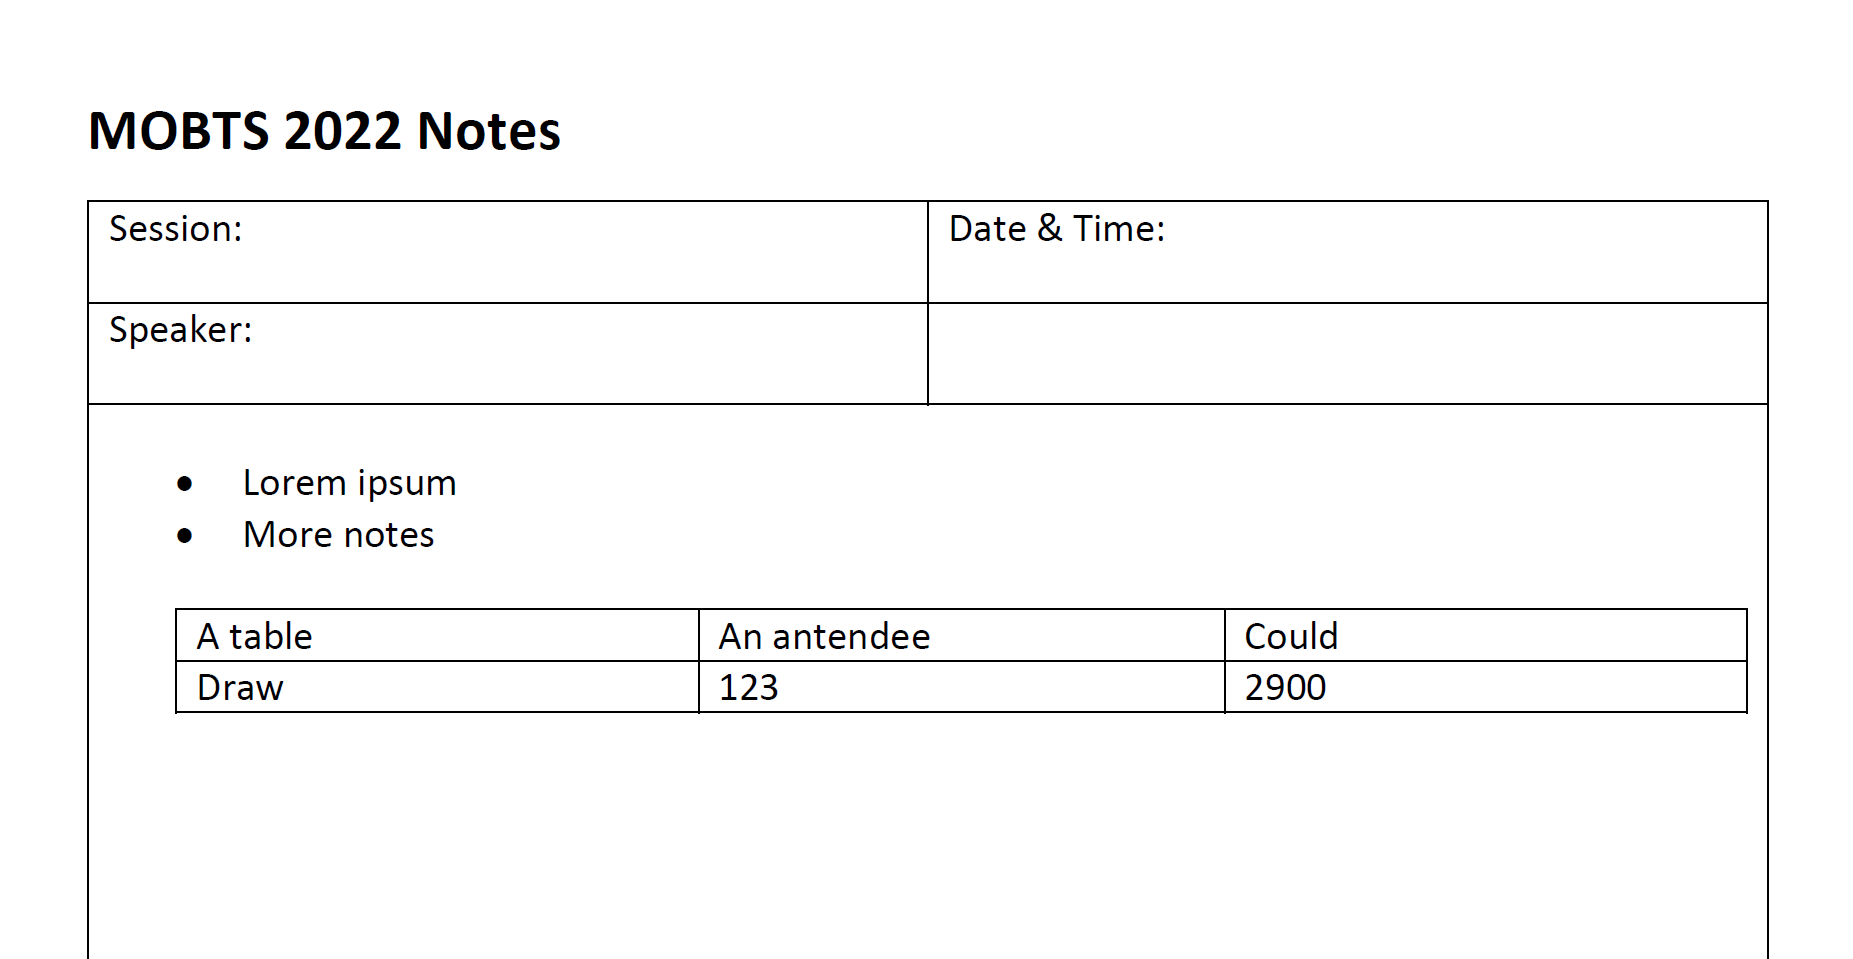
\includegraphics[width=0.9\textwidth]{img/notes_template.PNG}
    
    \end{center}
    \caption{Vereinfache Notizen Vorlage}
    \label{fig:notes-template}
\end{figure}

Da aufgrund der gegenwärtigen Situation ein Teil der Konferenz digital stattfinden wird ist davon auszugehen, dass Vortrage uns andere Session wenigstens zu einem gewissen Grad auch aufgezeichnet werden.
Wie oder wo diese Aufzeichnungen zugänglich sein werden, ist allerdings unklar, womit auch das (digitale) Auffinden von Ressourcen nich klar organisiert zu sein scheint. 

\subsection{Anforderungen}
Aus der dargelegten Problembeschreibung soll zunächst eine high-level Vision für eine mögliche App abgeleitet werden.
Als grundlegendes Problem kann hier eine fehlende Digitalisierung der Konferenzressourcen und eine fehlden zentralisiertung identifiziert werden.
Wichtige Dokumente werden ausgedruckt verwendet und Informationen sind nicht einfach zentral an einem Ort abrufbar.
Die Idee einer App stellt sich also in der Beantwortung der Frage \enquote{Wo finde ich X?} mit \enquote{In der \ac{MOBTS} App.} dar.
Alle relevanten Informationen die vor, während und nach der Konferenz benötigt werden, sollen an einem einzigen Punkt einfach zugänglich gemacht werden.

\subsubsection*{Vor der Konferenz}
\textbf{Allgemeine Informationen} zu den \ac{MOBTS} Konferenzen, Neuigkeiten und sonstige Inhalte, die gegnwärtig auf der Website der \ac{MOBTS} \url{https://mobts.org/} angeboten werden, sollen in der App einsehbar sein.
So sollen sich Interessenten und mögliche Besucher einfach einen Überblick verschaffen können.

\textbf{Tickets} und Informationen zum Besuch der \ac{MOBTS} sollen auch in der App verfügbar sein.
Denkbar hier ist, dass bei Erwerb eines Ticket ein Nutzeraccount in der App angelegt wird, über den der Besucher sein Ticket speichern kann und auf weitere Informationen zur Konferenz zugreifen kann.
Die App kann das gespeichert Ticket bei Anmeldung am Konferenzort in Form eines QR-Codes oder durch \ac{NFC} nutzen, um den Besucher zu identifizieren und eine Badge auszustellen.
So entfällt die Notwendigkeit ein Ticket ausdrucken und mitbringen zu müssen.
Außerdem ist so gesichert, dass die Tickets zentral auf der Infrastruktur der MOBTS gesiepchert sind, wodurch in Problemfällen einfach gehandelt werden kann.
Klappt die Anmeldung über die mobile App beispielsweise nicht, so ist es denkbar, dass sich der Besucher über einen Webbrowser anmeldet und dort Zugriff auf die selben Unterlagen wie in der App hat.
Dank moderner Entwicklungstechnologien ist die Bereitstellung einer Website mit nur geringfügig größerem Aufwand als die einer App verbunden.

\subsubsection*{Während der Konferenz}
\textbf{Informationen} über den Verlauf und die Örtlichkeiten der einzelnen Veranstaltungen sollen in App zugänglich gemacht werden.
Das soll verhindern, dass Besucher der Konferenz Informationen am Konferenzort suchen müssen, oder ihre eigenen Ausdrucke der Pläne mitbringen, welche eventuelle Änderungen nicht abbilden.
Beide Fälle würden am Konferenztag für vermeidbare Probleme sorgen, die einfach umgangen werden können, wenn alle relevanten Informationen in einer App zugänglich sind.

\textbf{Virtuelle Sessions} sollen idealerweise über die App oder eine Website zugänglich sein. 
Da aber in \autoref{ch:conference-systems} bereits dargelegt wurde, dass vermutlich Konferenzsysteme dritter für die virtuelle Ausführung der Sessions verwendet werden, ist dies unter Umständen nicht möglich.
Daher soll als Mindestanforderung über die App Zugang zu besagten System möglich sein, etwa durch das anklicken eines Buttons, eines Links oder des Auffindens von Anmelde- und Einwahlinformationen.

\textbf{Notizen} und Vorlagen für das Aufschreiben von Notizen sollen ebenfalls über die App möglich und zugänglich sein.
Vorteilhaft hier ist, dass einer App die einzelnen Sessions, deren Speaker und Uhrzeiten bereits bekannt sind, wodurch diese auf einem Template wie in \autoref{fig:notes-template} bereits ausgefüllt werden können.
Hier muss allerdings auch bedacht werden, dass diese bereits vorausgefüllten Vorlagen als Download und somit zum Ausdrucken bereitstehen müssen, da das Schreiben von Notizen auf einem Smartphone für die meisten Besucher vermutlich nicht der bevorzugte Weg sein wird.
Gleichzeitig soll hier aber auch auf die Vorteile einer eventuellen Website hingewiesen sein, die gleiches ermöglichen kann.
Das Schrieben auf einem Laptop gestaltet sich als sehr viel angenehmer als auf einem Handy.
Vorteil des digitalen Notizen Schreibens ist, dass Notizen mit einem Nutzeraccount assoiziiert werden können und in der App direkt neben Ressourcen zu den jeweiligen Sessions dargestellt sind.

\textbf{Interaktion mit den Speakern} in virtuellen Sessions ist auf mehrere Wegen denkbar, entweder werden die Möglichkeiten der Konferenzsysteme, wie etwa Chats, genutzt, oder es werden eigene Interaktionsmöglichkeiten über die eigene App geschaffen, durch die beispielsweise Fragen gestellt und von anderen Besuchern Hochgewählt werden können.

\subsubsection*{Nach der Konferenz}
\textbf{Notizen und Ressourcen} zu den einzelnen Sessions sollen auch nach der Konferenz leicht in der App zugänglich sein.
Dies soll Teilnehmenden ermöglich, nach Ende der Konferenz die Themen wieder aufzuarbeiteten.
Allgemein sollen Ressourcen vergangener Konferenzen über den Nutzeraccount gespeichert werden, sodass bei erneutem Konferenzbesuch einfach auf alte Notizen zurückgegriffen werden kann.
Die App funktioniert dabei als Single Point of Contact, über den auch mehrfache Besucher ihre Erlebnisse auf der \ac{MOBTS} Konferenz organisieren köknnen.

\textbf{Umfragen} und ähnliche Feeback Möglichkeiten, sowie wege der Kontaktaufnahme mit den Organisierern, etwa über Kontaktfomulare sollen auch über die App zugänglich gemacht werden.
So können Besucher der Konferenz auch nach Ende der Konferenz die App als zentralen Punkt der Interaktion mit Konferenzressourcen nutzen.
 
\subsection{Architektur}
\begin{figure}[h]
    \begin{center}
        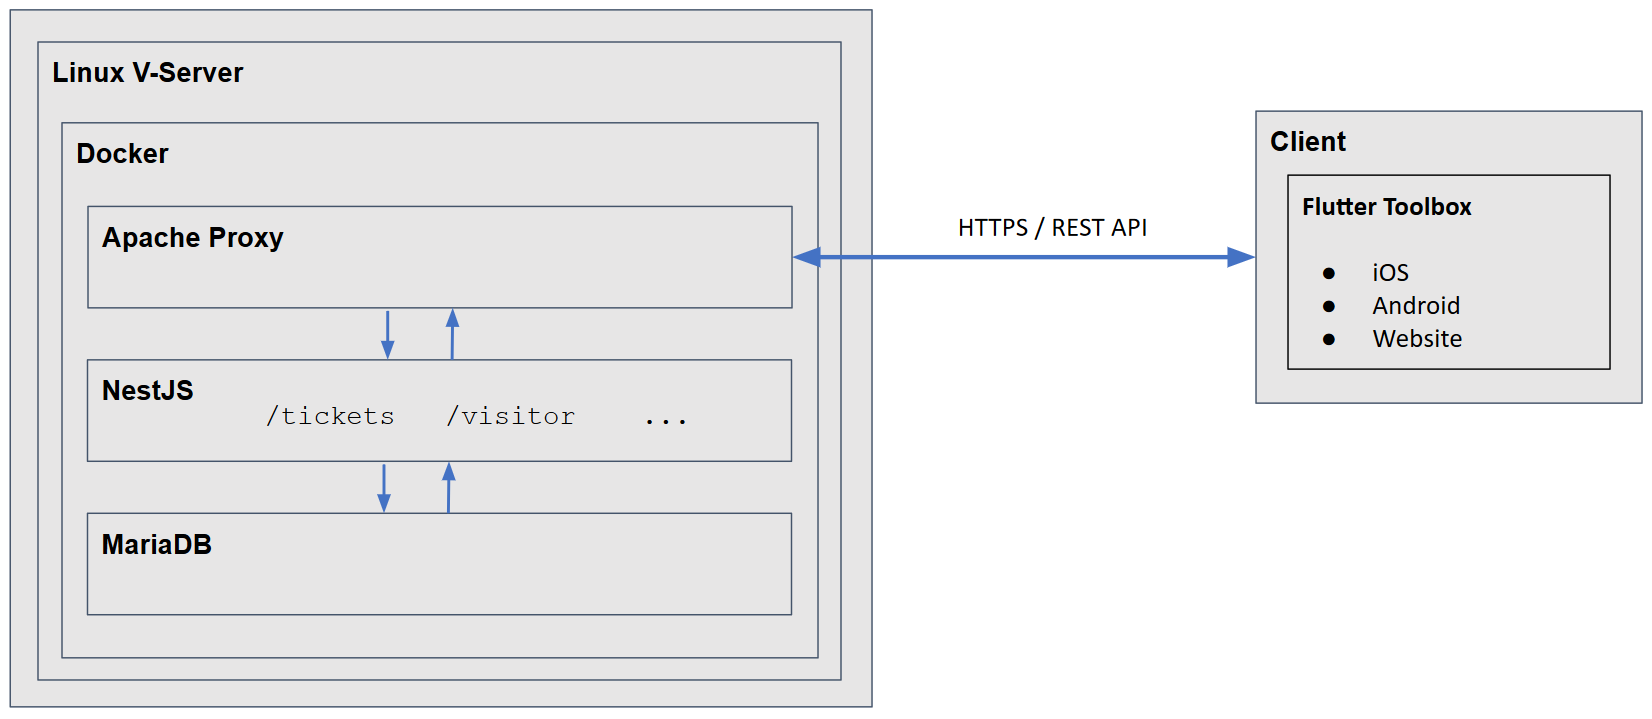
\includegraphics[width=0.9\textwidth]{img/app_architecture.PNG}
    \end{center}
    \caption{Mögliche Architektur einer App für die MOBTS Konferenz}
    \label{fig:architecture}
\end{figure}

\autoref{fig:architecture} zeigt eine Übersicht zu einer möglichen Architektur der App.
Ein Client kommuniziert hier über eine \ac{REST} \ac{API} mit einem Server.
Dabei kann der Client hier sowohl eine Website, als auch eine native Adnroid oder iOS App sein.
Auf dem Server läuft in einem Container ein Proxy, der Anfragen an den Server an die zuständigen Komponenten deligiert.
Der Komponent, der die meisten Anfragen verarbeiten wird, ist eine Node.js Laufzeit Umgebung, auf der ein NestJS Server läuft.
Hier ist die Logik der App implementiert -- Anfragen werden verarbeitet, Daten geladen und gespeichert und Berechtigung überprüft.
Um für Persistenz der Daten zu sorgen läuft in dem Container auch eine Datenbank, in Falle der dargestellten Architektur eine MariaDB, mit der die Node.js Laufzeitumgebung kommuniziert, um Daten zu laden und zu speichern.

\subsection{Technologien}
\subsubsection*{Flutter}
Flutter ist eine von Goolge entwickelte Technologie, die als Werkzeug zur Entwicklung nativer Android und iOS Anwendungen verwendete werden kann.
Dabei müssen Entwickler lediglich einen Code entwickeln, welcher dann von Flutter zu jeweils nativen Android und iOS Applikationen kompiliert wird.
Weiterhin bietet die neuste Version, Flutter 2, erweiterte Möglichkeiten bezüglich der Webeinbindung.
Entwickelte Apps können so einfach auch als Webanwendung bereitgestellt werden.
Damit werden auch nutzer angesprochen, die sich nur für die Konferenz keine App herunterladen wollen. \autocite{B_GoogleDevelopers.} 

\subsubsection*{\ac{REST} \ac{API}}
Eine \ac{API} bezeichnet eine Schnittstelle zwischen Programmen. 
Im Falle der App Entwicklung wir hier primär die Schnittstelle zwischen Back- und Frontend genauerer Betrachtung erfordern.
Grundlegend ist das Backend (der Server) dafür veranwortlich die Logik einer Anwndung, sowie die Datenverarbeitung bereitszustellen.
Diese beinhalten beispielsweise das Anlegen von Nutzerkonten, Authorisierungskonzepte, beispielsweise über Sessions, und Speichern von Daten.
Das Frontend (die App) ist die Schnittstelle zum Endnutzer, über die mit der Anwendung kommuniziert und interagiert wird.
Dabei ist es Aufgabe der App, Informationen des Servers dem Nutzer anzuzeigen und Eingaben des Nutzers an den Server zu senden. 
Dies geschiet wiederum über die \ac{API}.

\ac{REST} bezeichnet das Architekturprinzip einer API.
Zwar gibt es hier grundlegend keine standardisierte Methoden oder Prinzipien, es können aber einige Kritierien dargelegt werden.
Grundsätzlich setzt eine \ac{REST} \ac{API} eine zustandslose Client/Server-Kommunkation um, was bedeutet, dass es keine gegebene Verbindung zwischen einzelnen Anfragen gibt, wodurch jede Anfrage beispielsweise neu Authentifiziert und Authorisiert werden muss \autocite{B_RedHat.}.

\begin{figure}[h]
    \begin{center}
        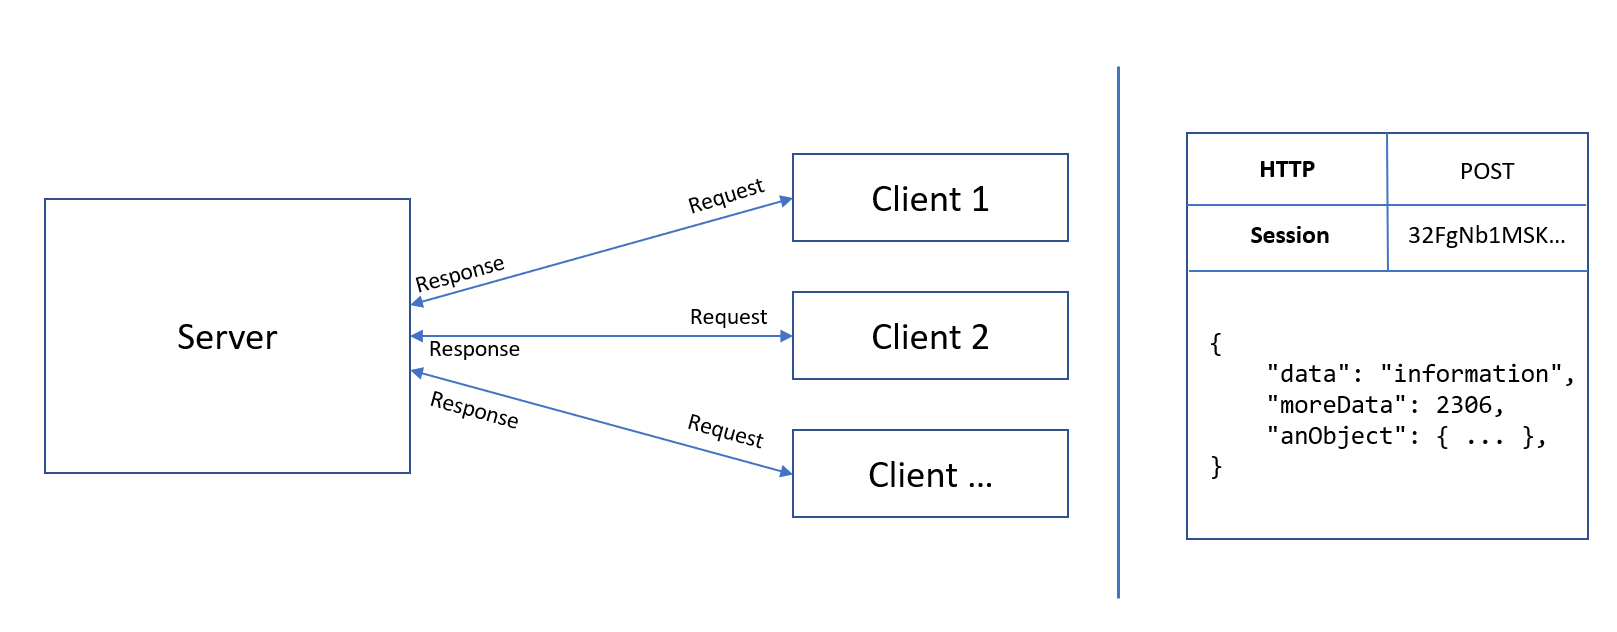
\includegraphics[width=0.9\textwidth]{img/rest_api.PNG}
    \end{center}
    \caption{Grundlegendes Konzept einer REST API}
    \label{fig:rest-api}
\end{figure}

\autoref{fig:rest-api} zeigt vereinfacht das Schema einer \ac{REST} \ac{API}, in der mehrere Clients andfragen an einen Server schicken, welche jeweils mit einer Antwort des Servers beantwortet werden.

\subsubsection*{Docker}
Docker bezeichnet eine beliebte Softwarelösung zur Containerization von Anwendungen.
Containerization bezeichnet dabei das Prinzip Teile einer Anwndung oder eine gesamte Anwendung mit allen Abhängigkeiten, wie externen Code-Bibliotheken ein einem Paket einzukapseln.
Ein häufig auftretendes Problem der Software Entwicklung ist, dass Software zwar auf einem System läuft, auf einem anderen aber nicht.
Das ist in sofern problematisch, da Anwender und Unternehmen darauf vertrauen müssen, dass Anwendungen auf allen Systemen gleich laufen.
Um dieses Problem zu lösen, muss entweder ein hoher Aufwand in die Konfiguration von Systemen gesteckt werden, oder das Vertrauen von Anwendern und Unternehmen muss betrogen werden.

Containerization löst dies, indem es das Problem nicht auftreten lässt.
Durch einbindung aller Abhängigkeiten läuft eine Anwendung auf allen Systemen gleich und es bedarf nur eines geringen Konfigurationsaufwands \autocite{B_IBMCloudEducation.2019}.

Docker stellt dabei eine beliebte Lösung der Containerization dar.
Nach einer Umfrage von IBM verwenden bis zu 60\% der Befragten Docker als eine Deployment Platform \autocite{B_IBMCloud.}.
Vorteilhaft an der Verwendung von Mainstream Technologien ist die Existenz eine großen Community und weitereichender Ressourcen zum Anlernen der Technologie.
Auftretende Probleme können auch aufgrund einer größeren Community schnell gelöst werden. 

\subsubsection*{Node.js}
Node.js ist nach eigener Angabe eine asynchrone ereignisgesteuerte JavaScript Laufzeitumgebung. \autocite{Node.js.}
Das bedeutet, dass so wie in einem Webbrowser, in Node.js JavaScript Code ausgeführt werden kann.
Dabei ist Node.js besonders für das entwickeln von Servern ausgelegt.
Vorteilhaft gegenüber anderer Sprachen ist bei der Entwicklung von JavaScript Servern mit Node.js vor allem die große Community, die sich um Node.js gebildet hat.
Große Communities sind dann immer hilfreich, wenn Probleme auftreten, da entweder Ressourcen im Überfluss zur Verfügung stehen, oder Fragen in Foren schnell von aktiven Vertretern der Community beantwortet werden.
Laut der jährlichen Entwicklerumfrage des Portals Stackoverflow\footnotetext{\url{https://stackoverflow.com/}} verwenden bis zu 50\% aller Befragten Node.js in ihren Projekten -- sowohl privat als auch beruflich \autocite{B_Stackoverflow.2020}.

Weiterhin existieren für Node.js zahlreiche exteren Code Bibliotheken, die den Entwicklungsprozess signifikant beschleunigen.
Ebenso gibt es eine große Anzahl an Frameworks, die die Serverentwicklung zu einem gewissen Grad abstrahieren und somit wiederum den Entwicklungsprozess vereinfachen können.
Insbesondere die Auswahl eines passenden Frameworks entscheidet bei der Arbeit mit Node.js über die tatsächliche Umsetzung einer App.

\subsubsection*{NestJS}
NestJS ist ein Node.js basiertes Framework \autocite{B_NestJs.}.
Es ist auf eine Trennung von logisch unabhängigen Programmkomponenten ausgelegt.
Durch diese Entzerrung bleibt eine Anwendung, auch dann wenn sie umfangreicher wird, immernoch übersichtlich.
Grundlegend unterteilt NestJS einen jeweiligen Teil der Geschäftslogik in folgende Komponenten ein:
\begin{itemize}
    \item \textbf{Controller} sind für das Request/Response Handling verantwortlich, also die Kommunikation mit den Clients
    \item \textbf{Provider} (Services) sind für die tatsächliche Geschäftslogik veranwortlich. Hier werden die Anfragen der Client verarbeitet und Anworten mit entsprechenden Daten gefüllt.
    \item \textbf{Modules} bieten schließlich die Schnittstelle ziwschen den Komponenten einer NestJS Anwendung.
\end{itemize}
Neben einer übersichtlichen Designphilosophie bietet NestJS weiterhin einen nativ die Unterstützung der Programmiersprache TypeScript.
TypeScript ist eine Erweiterung der beliebtesten Srache zur Webentwicklung JavaScript, welche ebenso beliebt wie auch gefürchtet ist \autocite{B_Stackoverflow.2020}.
Gegenüber JavaScript bietet TypeScript den Vorteil, dass eine statische Typisierung von Valriablen das Entwickeln einfacher macht, da semantische Fehler im Code schneller gefunden und behoben werden können.
Da TypeScript auf JavaScript basiert, ist auch die Lernprozess für Programmierer, die noch nicht mit der Sprache vertraut sind, sehr linear und einfach.
Der Syntax beider Sprachen ist der gleiche, wodurch bereits in JavaScript Gelerntes direkt angewendet werden kann.

\subsubsection*{Datenbank}
Für die praktische Umsetzung einer App für die MOBTS 2022 gilt es in irgendeiner Form Daten zu speichern.
In der Informatik ist die dafür etablierte Lösung in fast jedem Falle eine Datenbank.
Für die meisten Anwendungsfälle etablierte sich in den letzten Jahrzehnten die relationale Datenbank als Standard.
In einer relationalen Datenbank werden Daten nach einem vorher festgelegtem Schema gespeichert \autocite{B_AWS.o.J.}.
Dieses Schema wird im Vorlauf in Form eines ER-Diagramms (Entity Relationship) dargestellt.
Die genaue Struktur eines solchen Diagramms kann erst dann erstellt werden, wenn die praktische Implementierung der App genauer durchdacht wird.
Da diese aber in jedem Fall nicht so weit vom \enquote{normalen} Anwendungsfall abweichen wird, sollte eine relationale Datenbank die richtige Wahl sein.
An dieser Stelle sei daher eine relationale, SQL-basierte Datenbank empfohlen, ohne, dass genauer auf deren Strukturierung eingegangen werden soll.
Für die Wahl eines konkreten Datenbankmanagementsystems sei an dieser Stelle MariaDB oder PostgreSQL empfohlen -- beides sind populäre Lösungen, die aus vorher bereits genannten Gründen den Entwicklungsprozess vereinfachen können.

\section{Fazit}

% END OF ACTUAL CONTENT --------------------------




\printbibliography[title=Literaturverzeichnis]
\cleardoublepage

% Der Anhang beginnt hier - jedes Kapitel wird alphabetisch aufgezählt. (Anhang A, B usw.)
\appendix
\ihead{\appendixname~\thechapter} % Neue Header-Definition

% appendix.tex einziehen
\chapter{Vorgeschlagene Konferenzthemen}
\label{app:konferenzthemen}
\begin{itemize}
	\item Motivation im digitalen Zeitalter
	\item Gamification
	\item Learning @ Business
	\item Moocs / Online Corporate Learning
	\item Social / Personal Development im online Zeitalter
	\item Digital Schools
	\item Digital Learning @ DHBW
	\item Remote Working
	\item Duale Ausbildung International
	\item Digitalisierung in der Hochschule in Bezug auf Corona
	\item Pädagogik für Dozenten
	\item Studentenmotivation in der Hochschule
	\item Organisation einer Hochschule
	\item Paper Writing Erfahrungsaustausch
\end{itemize}

\chapter{Umfrage}
\label{app:umfrage}
\begin{figure}[h]
	\centering
	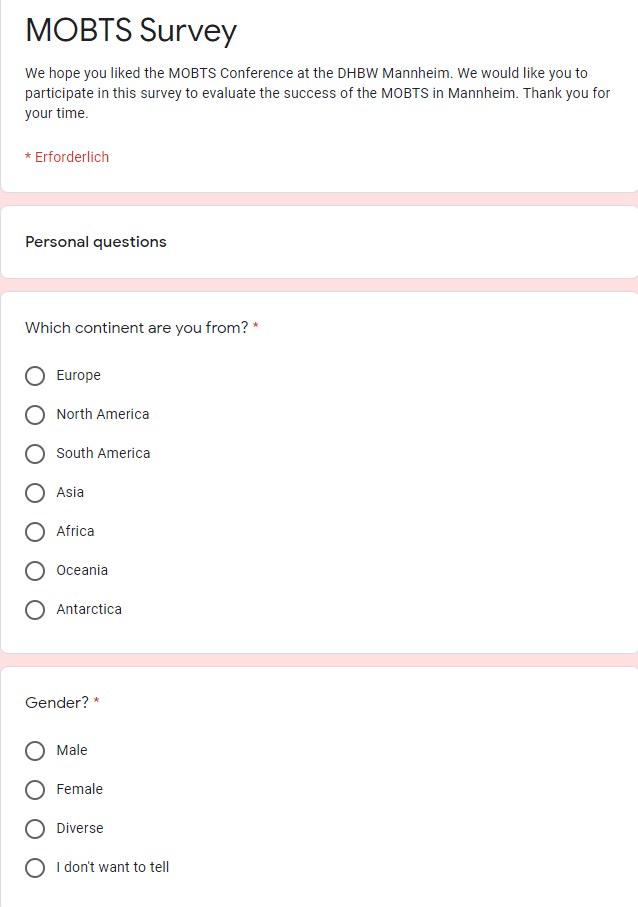
\includegraphics[width=10 cm]{img/survey1.png}
	\caption[MOBTS Umfrage]{MOBTS Umfrage Teil 1}
	\label{fig:survey1}
\end{figure}

\begin{figure}[h]
	\centering
	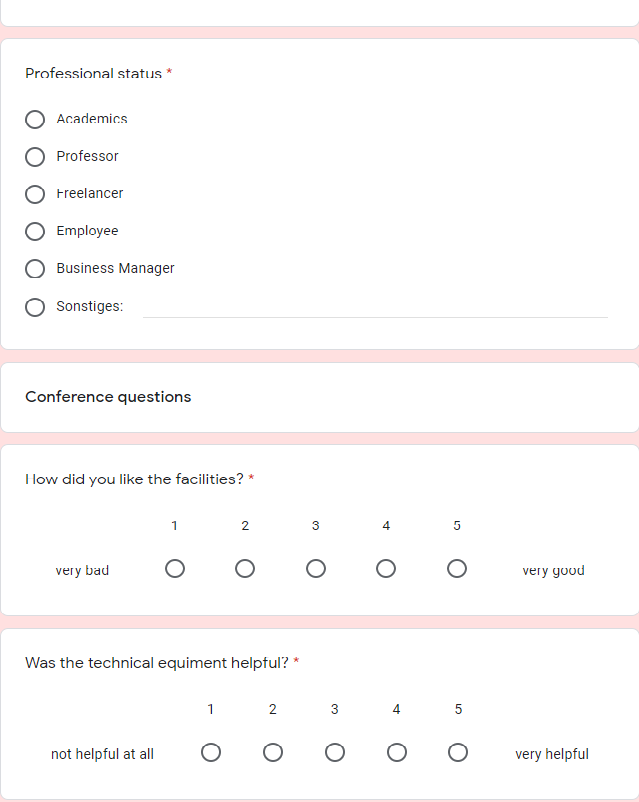
\includegraphics[width=10 cm]{img/survey2.png}
	\caption[MOBTS Umfrage]{MOBTS Umfrage Teil 2}
	\label{fig:survey2}
\end{figure}

\begin{figure}[h]
	\centering
	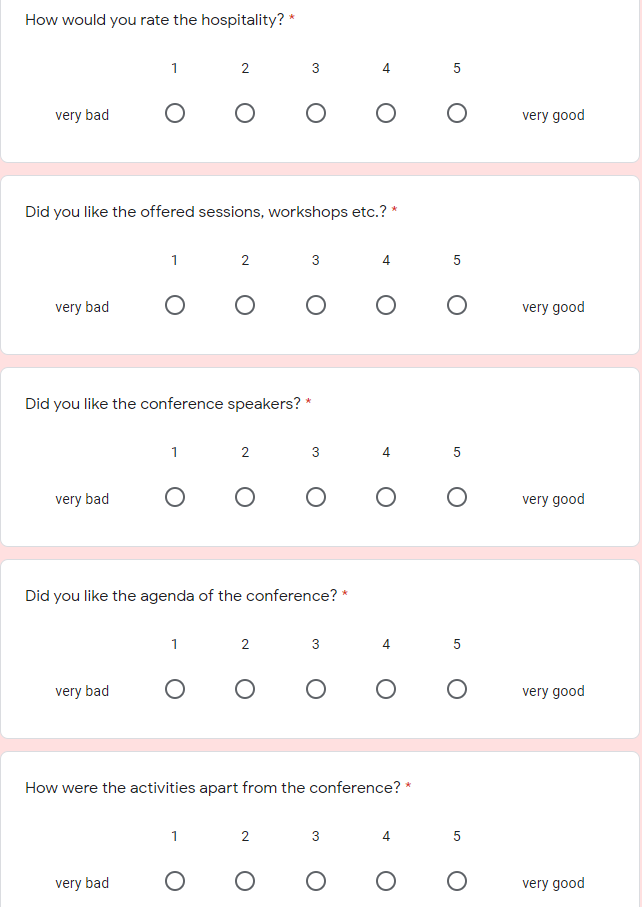
\includegraphics[width=10 cm]{img/survey3.png}
	\caption[MOBTS Umfrage]{MOBTS Umfrage Teil 3}
	\label{fig:survey3}
\end{figure}

\begin{figure}[h]
	\centering
	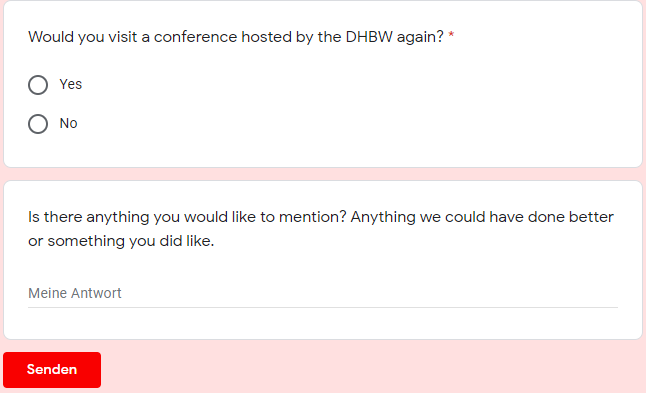
\includegraphics[width=10 cm]{img/survey4.png}
	\caption[MOBTS Umfrage]{MOBTS Umfrage Teil 4}
	\label{fig:survey4}
\end{figure}

\chapter{Catering-Angebot}
\label{app:angebot}

%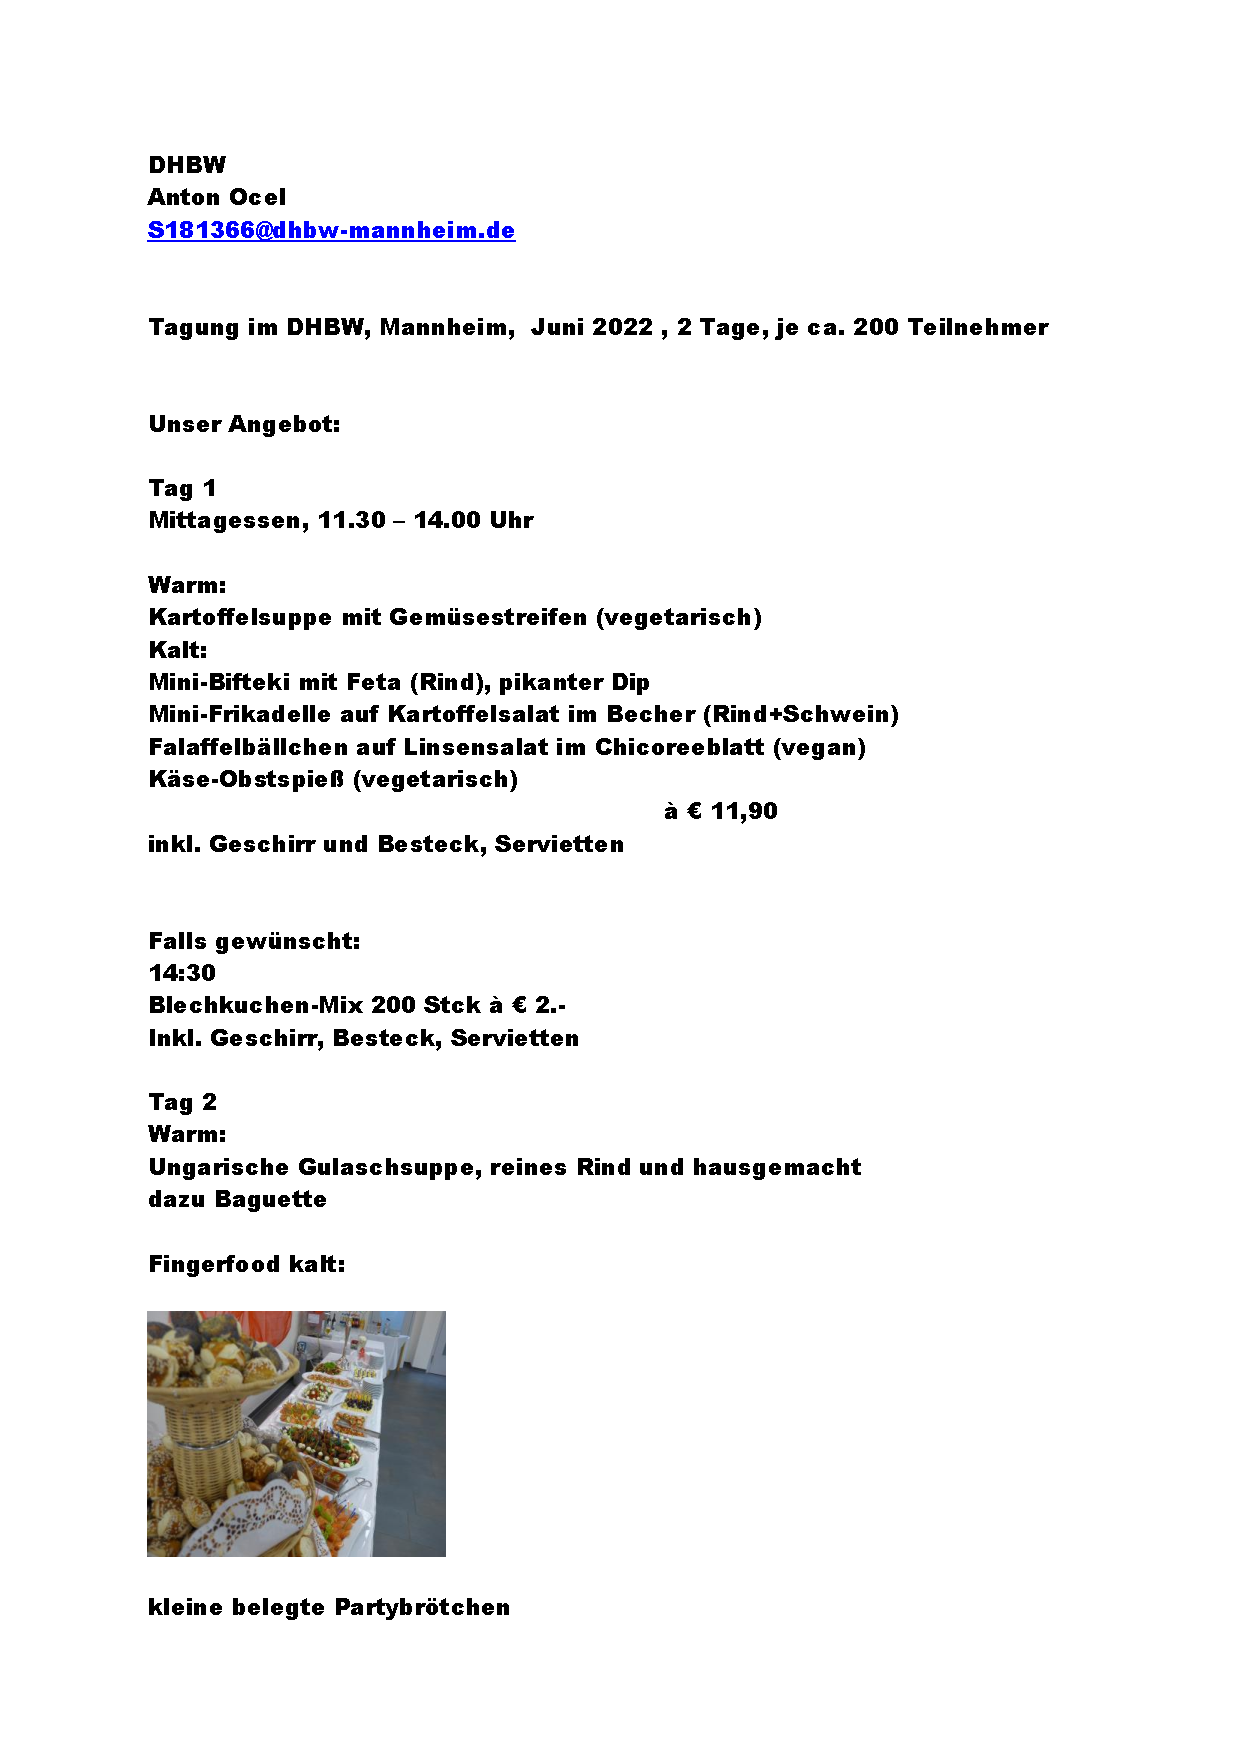
\includepdf[pages=1]{DHBWOcel2x200p22.pdf}



% Ehrenwörtliche Erklärung ewerkl.tex einziehen
% !TEX root =  master.tex

\clearpage
\chapter*{Ehrenwörtliche Erklärung}

% Wird die folgende Zeile auskommentiert, erscheint die ehrenwörtliche
% Erklärung im Inhaltsverzeichnis.

% \addcontentsline{toc}{chapter}{Ehrenwörtliche Erklärung}
Ich versichere hiermit, dass ich die vorliegende Arbeit
 mit dem Thema: \textit{\DerTitelDerArbeit} selbstständig verfasst und keine anderen als die angegebenen Quellen und
Hilfsmittel benutzt habe. Ich versichere zudem,
dass die eingereichte elektronische Fassung mit der gedruckten Fassung übereinstimmt.

\vspace{3cm}
Ort, Datum \hfill \DerAutorDerArbeit



\end{document}